Likewise, define properties/axioms for the structure of $\R$.

\subsection{Fields}

\begin{definition}{Field}{field}
  A \textbf{field} is a set $\mathbb{F}$ with two binary operations:
  \[
    +\colon\mathbb{F}\times\mathbb{F}\to\mathbb{F}
    \quad\text{(plus)},\qquad
    \cdot\colon\mathbb{F}\times\mathbb{F}\to\mathbb{F}
    \quad\text{(times)},
  \]
  with axioms:
  \begin{enumerate}[leftmargin=3em]
    \item[(A1)] \textbf{Additive associativity:}
          \[
            a+(b+c)=(a+b)+c\qquad\forall a,b,c\in\mathbb{F}.
          \]
    \item[(A2)] \textbf{Additive commutativity:}
          \[
            a+b=b+a\qquad\forall a,b\in\mathbb{F}.
          \]
    \item[(A3)] \textbf{Additive identity:}
          \[
            \exists 0\in\mathbb{F}\text{ such that }\forall a\in\mathbb{F},\quad a+0=a.
          \]
    \item[(A4)] \textbf{Additive inverses:}
          \[
            \forall a\in\mathbb{F},\quad\exists -a\in\mathbb{F}\text{ such that }a+(-a)=0.
          \]
    \item[(M1)] \textbf{Multiplicative associativity:}
          \[
            a\cdot(b\cdot c)=(a\cdot b)\cdot c\qquad\forall a,b,c\in\mathbb{F}.
          \]
    \item[(M2)] \textbf{Multiplicative commutativity:}
          \[
            a\cdot b=b\cdot a\qquad\forall a,b\in\mathbb{F}.
          \]
    \item[(M3)] \textbf{Multiplicative identity:}
          \[
            \exists 1\in\mathbb{F}\text{ such that }\forall a\in\mathbb{F},\quad a\cdot1=a.
          \]
    \item[(M4)] \textbf{Multiplicative inverses:}
          \[
            \forall a\in\mathbb{F},\quad a\ne0\implies
            \exists a^{-1}\in\mathbb{F}\text{ such that }a\cdot a^{-1}=1.
          \]
    \item[(D)] \textbf{Distributivity:}
          \[
            a\cdot(b+c)=(a\cdot b)+(a\cdot c)\qquad\forall a,b,c\in\mathbb{F}.
          \]
  \end{enumerate}
\end{definition}

\begin{example}
  \begin{itemize}
    \item $(\Q,+,\cdot)$ is a field.
    \item $(\N,+,\cdot)$ is not a field: it fails (A3), (A4), and (M4).
    \item $(\Z\bmod 2,+,\cdot)$ is a field.
  \end{itemize}
\end{example}

\begin{example}[Multiplication by Zero]
  For a field $(\mathbb{F},+,\cdot)$,
  \[
    \forall a\in\mathbb{F},\qquad a\cdot0=0.
  \]
  \begin{proof}
    (i)
    \begin{align*}
      a\cdot0 & = a\cdot(0+0)     &  & \text{(additive identity)} \\
              & = a\cdot0+a\cdot0 &  & \text{(distributivity)}
    \end{align*}
    (ii)
    \begin{align*}
      0 & = (a\cdot0)+(-(a\cdot0))             &  & \text{(additive inverse)}           \\
        & = ((a\cdot0)+(a\cdot0))+(-(a\cdot0)) &  & \text{(i)}                          \\
        & = (a\cdot0)+((a\cdot0)+(-(a\cdot0))) &  & \text{(additive associativity)}     \\
        & = (a\cdot0)+0                        &  & \text{(additive inverse)}           \\
        & = a\cdot0                            &  & \text{(additive identity).}\qedhere
    \end{align*}
  \end{proof}
\end{example}

\subsection{Ordering}

\begin{definition}{Ordered Field}{ordered-field}
  An \textbf{ordered field} is a field $\mathbb{F}$ with a relation $\le$ satisfying:
  \begin{enumerate}[leftmargin=3em]
    \item[(O1)] $\forall a,b\in\mathbb{F},\quad a\le b\text{ or }b\le a$.
    \item[(O2)] $a\le b\text{ and }b\le a\implies a=b$.
    \item[(O3)] $a\le b\text{ and }b\le c\implies a\le c$.
    \item[(O4)] $a\le b\implies\forall c\in\mathbb{F},\quad a+c\le b+c$.
    \item[(O5)] $a\le b\text{ and }0\le c\implies ac\le bc$.
  \end{enumerate}
\end{definition}

\begin{example}
  $(\Q,+,\cdot,\le)$ is an ordered field.
  $(\R,+,\cdot,\le)$ is an ordered field (more later).
\end{example}

In general, any ordered field contains a ``copy'' of $\N$, $\Z$, and $\Q$.

\begin{theorem}{Negation Reverses Order}{negation-reverses-order}
  Let $(\mathbb{F},+,\cdot,\le)$ be an ordered field. Then
  \[
    \forall a,b\in\mathbb{F},\qquad a\le b\implies -b\le-a.
  \]
\end{theorem}

\begin{proof}
  By (O4) of Definition~\ref{def:ordered-field},
  \[
    a\le b\implies a+(-a+(-b))\le b+(-a+(-b)).
  \]
  Using the field axioms (details skipped),
  \begin{align*}
    (a+(-a))+(-b) & \le(b+(-b))+(-a), \\
    0+(-b)        & \le0+(-a),        \\
    -b            & \le-a.\qedhere
  \end{align*}
\end{proof}

\subsection{Absolute Value}

\begin{definition}{Absolute Value}{absolute-value}
  For an ordered field $(\mathbb{F},+,\cdot,\le)$ and any $a\in\mathbb{F}$, the \textbf{absolute value} is
  \[
    \abs{a}:=
    \begin{cases}
      a,  & a\ge0,            \\
      -a, & \text{otherwise}.
    \end{cases}
  \]
\end{definition}

Intuition: $\abs{a}$ means the distance from $a$ to $0$.
\begin{center}
  \begin{tikzpicture}[>=latex]
    \draw[<->] (-2.5,0) -- (2.5,0) node[right] {$\mathbb{F}$};
    \draw (-0.8,0) -- (-0.8,0.15);
    \draw (0.8,0) -- (0.8,0.15);
    \node[below] at (-0.8,0) {$a$};
    \node[below] at (0.8,0) {$0$};
    \node at (0,-0.65) {$\underbrace{\hspace{1.6cm}}_{\abs{a}}$};
  \end{tikzpicture}
\end{center}

$\abs{a-b}$ means the distance from $a$ to $b$.
\begin{center}
  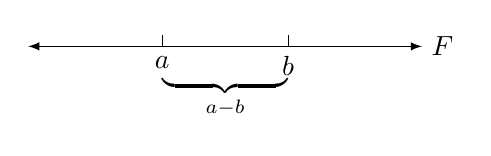
\begin{tikzpicture}[>=latex]
    \draw[<->] (-2.5,0) -- (2.5,0) node[right] {$\mathbb{F}$};
    \draw (-0.8,0) -- (-0.8,0.15);
    \draw (0.8,0) -- (0.8,0.15);
    \node[below] at (-0.8,0) {$a$};
    \node[below] at (0.8,0) {$b$};
    \node at (0,-0.65) {$\underbrace{\hspace{1.6cm}}_{\abs{a-b}}$};
  \end{tikzpicture}
\end{center}

\begin{theorem}{Properties of Absolute Value}{absolute-value-properties}
  For an ordered field $(\mathbb{F},+,\cdot,\le)$:
  \begin{enumerate}[label=(\roman*)]
    \item $\abs{a}\ge0,\quad\forall a\in\mathbb{F}$.
    \item $\abs{ab}=\abs{a}\cdot\abs{b},\quad\forall a,b\in\mathbb{F}$.
    \item \textbf{Important (triangle inequality):}
          \[
            \abs{a+b}\le\abs{a}+\abs{b},\qquad\forall a,b\in\mathbb{F}.
          \]
  \end{enumerate}
\end{theorem}
